% airgap-rca: working manuscript template. Compile with pdfLaTeX.
% All experimental outcomes are pending. Do not replace placeholders by hand.
\documentclass[conference]{IEEEtran}
\usepackage[T1]{fontenc}
\usepackage{amsmath,amssymb}
\usepackage{graphicx,booktabs,array,tabularx}
\usepackage{xcolor,tikz}
\usetikzlibrary{arrows.meta,positioning,shapes.geometric}
\usepackage{listings}
\usepackage{xurl}
\usepackage[hidelinks]{hyperref}
\definecolor{accent}{HTML}{245A73}
\definecolor{pale}{HTML}{EDF3F6}
\newcommand{\system}{\textsc{airgap-rca}}
\newcommand{\pending}{\textcolor{accent}{\textit{Pending}}}
\newcommand{\draftnote}[1]{\par\smallskip\noindent\colorbox{pale}{\parbox{\dimexpr\columnwidth-2\fboxsep\relax}{\small\textbf{Draft task.} #1}}\par\smallskip}
\newcommand{\placeholder}[2]{\noindent\fbox{\parbox[c][#1][c]{0.94\columnwidth}{\centering\small\textcolor{accent}{#2}}}}
\newcolumntype{Y}{>{\raggedright\arraybackslash}X}
\lstset{basicstyle=\ttfamily\scriptsize,breaklines=true,columns=fullflexible,frame=single,rulecolor=\color{accent},showstringspaces=false}
\pagestyle{plain}
\begin{document}
\title{Sovereign Root Cause Analysis: Grounded Log Triage on Air-Gapped Edge Accelerators, with a Cross-Silicon Characterisation}
\author{\IEEEauthorblockN{Kayman Srinivasan}\IEEEauthorblockA{Working manuscript --- September 2026\\Affiliations and co-authors to be confirmed}}
\maketitle
\begin{abstract}
\textbf{Working abstract scaffold; results pending.} Engineering teams operating under strict data residency constraints need methods for investigating machine failures without exporting their logs. This project investigates a fully local log-triage pipeline that combines provenance-preserving ingestion, semantic and keyword retrieval, structured candidate generation, deterministic citation checks, and refusal when no candidate passes the evidence policy. The planned evaluation compares the pipeline on a Jetson AGX Orin and a Qualcomm RB3 Gen 2, documenting model, runtime, and quantisation differences. Quality evaluation will distinguish cause accuracy, citation integrity, refusal behaviour, and incorrect accepted answers. Performance evaluation will measure request latency, generation throughput, power, and energy per triage. Component ablations will examine the contribution of keyword matching, verification, and refusal. No implementation outcome, accelerator compatibility, or benchmark result is claimed in this scaffold. The final abstract will replace this text with the measured quality--performance trade-offs and the principal limitations of the completed study.
\end{abstract}
\begin{IEEEkeywords}
root cause analysis, log triage, air-gapped inference, retrieval-augmented generation, selective prediction, edge computing
\end{IEEEkeywords}

\section{Introduction}
Machine logs record events that can help engineers reconstruct the sequence leading to a failure. A useful triage assistant must locate relevant events, relate them to a specific question, and provide evidence that a human can inspect. In environments that prohibit external processing of engineering data, retrieval and generation must operate locally. This project treats disconnected execution as an experimental requirement.

The intended output is a short ranked list of supported candidate causes, not an unrestricted explanation. A recorded symptom does not necessarily establish a physical root cause. For example, a timeout alone cannot distinguish a disconnected network from an unresponsive service. The system must preserve this uncertainty and refuse questions that require absent evidence.

\subsection{Research questions}
\begin{itemize}
\item \textbf{RQ1: Reliability.} How often does the system accept an incorrect answer, and what coverage does it retain?
\item \textbf{RQ2: Component contribution.} How do hybrid retrieval, verification, and refusal change quality and latency?
\item \textbf{RQ3: Platform trade-offs.} Under documented, comparable settings, how do the two execution platforms differ in latency, throughput, and energy?
\end{itemize}

\subsection{Planned contributions and scope}
The planned contributions are a reproducible offline pipeline, a reviewed question-and-evidence evaluation set, and a cross-platform characterisation. These remain objectives until demonstrated. All study data will be public or synthetic. Fine-tuning, a chat interface, and autonomous recovery are outside the core study. Evaluation on general system logs will not establish accuracy on semiconductor continuity, scan, or BIST failures.
\draftnote{Week 1: substantiate the motivation with primary literature. Do not claim a percentage of debugging time or global novelty without supporting sources. Final introduction target: approximately one page.}

\section{Related Work}
\subsection{Log analysis and failure diagnosis}
Loghub provides public system-log collections and their provenance~\cite{loghub}. Candidate selection must distinguish anomaly labels from cause labels. In particular, the Hadoop dataset documents injected failure scenarios~\cite{hadoop}, but reported label inconsistencies require incident-level review~\cite{hadooplabels}. The dataset has not yet been accepted for this study.
\subsection{Evidence-grounded generation}
\draftnote{Weeks 2--3: add verified primary papers on retrieval-augmented generation, attribution, and abstention. Compare their evidence guarantees with this system. Separate citation existence, textual relevance, and causal correctness.}
\subsection{Offline inference and platform evaluation}
\draftnote{Weeks 2--4: review primary work on local inference and energy measurement. Describe the gap supported by that review; do not equate an IEEE layout with publication readiness.}

\section{System Design}
\subsection{Execution boundary and provenance}
Figure~\ref{fig:architecture} specifies the proposed flow. A connected staging machine prepares versioned assets; execution targets receive the bundle and run without a network connection. Raw logs remain immutable. Each chunk stores a source identifier, source checksum, inclusive original line range, and text. A stable line-numbering convention must be fixed before ingestion.

\begin{figure}[t]
\centering
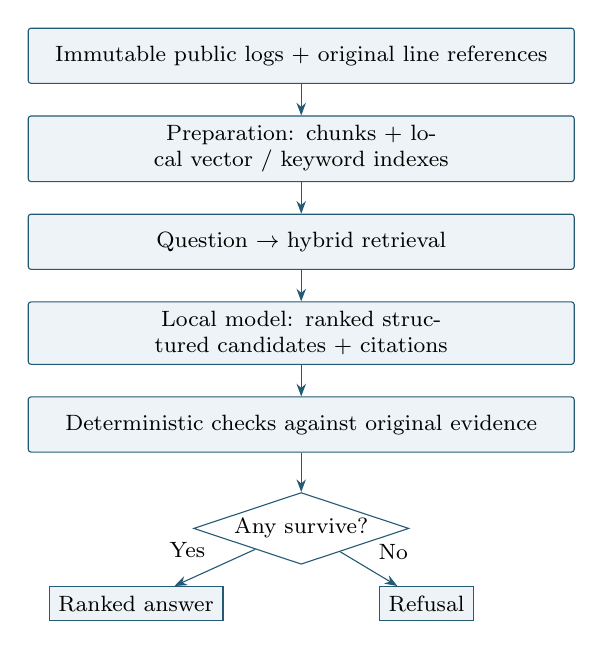
\begin{tikzpicture}[node distance=4mm, font=\footnotesize,
box/.style={draw=accent,rounded corners=1pt,align=center,text width=6.7cm,minimum height=7mm,fill=pale},
arr/.style={-{Stealth[length=1.6mm]},draw=accent}]
\node[box] (raw) {Immutable public logs + original line references};
\node[box,below=of raw] (idx) {Preparation: chunks + local vector / keyword indexes};
\node[box,below=of idx] (ret) {Question $\rightarrow$ hybrid retrieval};
\node[box,below=of ret] (gen) {Local model: ranked structured candidates + citations};
\node[box,below=of gen] (ver) {Deterministic checks against original evidence};
\node[draw=accent,diamond,aspect=3,align=center,below=5mm of ver,inner sep=1pt] (gate) {Any survive?};
\node[draw=accent,fill=pale,align=center,below left=5mm and 3mm of gate] (yes) {Ranked answer};
\node[draw=accent,fill=pale,align=center,below right=5mm and 3mm of gate] (no) {Refusal};
\draw[arr] (raw)--(idx); \draw[arr] (idx)--(ret); \draw[arr] (ret)--(gen); \draw[arr] (gen)--(ver); \draw[arr] (ver)--(gate);
\draw[arr] (gate)--node[above left]{Yes}(yes); \draw[arr] (gate)--node[above right]{No}(no);
\end{tikzpicture}
\caption{Proposed offline triage architecture. Verification uses original evidence, not generated text as its authority. This is a design figure, not evidence of implementation.}
\label{fig:architecture}
\end{figure}

\subsection{Local hybrid retrieval}
A local encoder maps chunks and the question to vectors. Keyword retrieval preserves sensitivity to exact error codes and identifiers. A possible deterministic fusion rule is reciprocal rank fusion:
\begin{equation}
S(c,q)=\frac{1}{\kappa+r_v(c,q)}+\frac{1}{\kappa+r_k(c,q)},
\label{eq:rrf}
\end{equation}
where $r_v$ and $r_k$ are one-based vector and keyword ranks. An absent result contributes zero. The fusion constant $\kappa$, retrieval depth, chunk size, and overlap are development choices, not benchmark-tuned settings. Equation~\ref{eq:rrf} is a proposed implementation choice; it is not a novelty claim. Add its primary reference if adopted.

\subsection{Structured generation}
The generator receives the question and retrieved evidence only. It returns at most three ranked candidates using a fixed schema. Each candidate separates the proposed cause from exact quoted evidence and references. Self-reported confidence is not treated as a calibrated probability.
\begin{lstlisting}[float=t,caption={Proposed output fields; schema illustration only.},label={lst:schema}]
{
  "status": "answer | refusal",
  "candidates": [{
    "rank": "integer",
    "cause": "narrow supported claim",
    "confidence": "optional uncalibrated score",
    "citations": [{
      "source_id": "allowed source identifier",
      "line_start": "original line number",
      "line_end": "original line number",
      "quote": "exact source text"
    }]
  }],
  "refusal_reason": "when applicable"
}
\end{lstlisting}
Listing~\ref{lst:schema} describes field types using strings; it is not an executable response or a formal JSON Schema. Parse failures must be logged. Logs are untrusted data, never instructions to the model or host.

\subsection{Deterministic verification and refusal}
For candidate $j$, define indicators for schema validity $s_j$, allowed-source membership $a_j$, valid line bounds $b_j$, quote fidelity $q_j$, and the fixed relevance policy $r_j$. A proposed gate is
\begin{equation}
V_j=s_j a_j b_j q_j r_j,\qquad
\mathrm{refuse}\ \text{if}\ \sum_j V_j=0.
\end{equation}
All citations and atomic claims in a retained candidate must satisfy the selected policy. Record each rejection reason and preserve surviving order. Exact-quote and line-bound checks establish integrity; term overlap does not prove entailment or causation. Cause correctness therefore requires independent evaluation. Execution failures must not be silently reclassified as successful refusals.
\draftnote{Week 3: specify the actual relevance rule, negation handling, multiple-citation policy, invalid-output policy, and any retry budget. Include examples the verifier mistakenly accepts.}

\section{Platforms and Experimental Setup}
\subsection{Hardware and execution configuration}
Populate Table~\ref{tab:hardware} from dated board inspection records. Confirm accelerator execution with runtime evidence and report CPU fallback. A successful process on a board does not establish NPU use. Match the base checkpoint, tokenizer, context budget, and decoding configuration. Report weight and activation precision and quantisation method; equal bit width alone is not equivalence.
\begin{table}[t]
\caption{Platform configuration record. No specifications verified yet.}
\label{tab:hardware}\centering\footnotesize
\begin{tabularx}{\columnwidth}{@{}Yll@{}}\toprule
Configuration & Jetson AGX Orin & RB3 Gen 2\\\midrule
Module, RAM, storage & \pending & \pending\\
OS, kernel, SDK & \pending & \pending\\
Runtime, backend & \pending & \pending\\
Checkpoint, tokenizer & \pending & \pending\\
Weights / activations & \pending & \pending\\
Quantisation method & \pending & \pending\\
Context / output budget & \pending & \pending\\
Power mode / clocks & \pending & \pending\\
Cooling / temperature & \pending & \pending\\
Power measurement & \pending & \pending\\\bottomrule
\end{tabularx}
\end{table}

\subsection{Dataset and answer-key construction}
Review candidate public datasets before freezing the test set. Store the dataset release, download source, license or usage terms, checksum, and selected incident IDs. Each evaluation item needs an answerability label, accepted cause descriptions, exact evidence lines, and a review rationale. Cause labels must not be indexed as evidence.

The proposed target is at least 50 answerable questions plus at least 10 refusal cases, subject to sufficient independently reviewed incidents. These are design targets, not achieved counts. Split development and evaluation by incident rather than by question wording. Report repeated questions from a common incident as related observations. Use original contiguous logs for final citation mapping rather than assuming a parsing sample preserves incident context.

Refusal cases should include missing causal evidence, symptoms compatible with several explanations, and questions about absent components. If evidence is deliberately removed, record the transformation and score that case separately. Report dataset-specific outcomes when more than one source is used.
\draftnote{Weeks 2--3: insert the reviewed case counts, incident counts, cause taxonomy, review process, disagreements, and dataset exclusions. If semiconductor examples are synthetic, label and analyse them separately.}

\subsection{Quality metrics and denominators}
Let $N$ denote all frozen questions, $N_A$ answerable questions, and $N_U$ unanswerable questions. For question $i$, let $a_i$ indicate an accepted answer, $r_i$ a refusal, and $e_i$ an execution error, with $a_i+r_i+e_i=1$. Let $z_i$ indicate answerability and $c_i^{(k)}$ indicate that a reviewed correct cause appears in the first $k$ returned candidates. Refusals and errors have $c_i^{(k)}=0$.
\begin{align}
\mathrm{Acc@}k &= \frac{\sum_i z_i c_i^{(k)}}{N_A},\quad k\in\{1,3\},\\
\mathrm{FAR} &= \frac{\sum_i a_i(1-c_i^{(1)})}{N},\\
\mathrm{AnsweredError} &= \frac{\sum_i a_i(1-c_i^{(1)})}{\sum_i a_i},\\
\mathrm{Coverage} &= \frac{\sum_i a_i}{N},\qquad
\mathrm{RefusalRate}=\frac{\sum_i r_i}{N},\\
\mathrm{CorrectRefusal} &= \frac{\sum_i(1-z_i)r_i}{N_U}.
\end{align}
An accepted answer on an unanswerable case is wrong under the reviewed policy. A zero denominator is reported as not applicable, never zero. Also report execution-error rate and the fraction of answered questions containing any incorrect candidate, even when the first cause is correct. The exact scoring policy remains to be agreed before evaluation.

For generated citations $C_g$ and citations passing the verifier $C_v$,
\begin{equation}
\mathrm{CitationPassRate}=\frac{|C_v|}{|C_g|}.
\end{equation}
Report this before filtering and report post-filter integrity separately. Call it a verifier pass rate unless independent review supports a stronger validity claim. Pair FAR with coverage to expose a system that obtains few errors by refusing almost everything. Include uncertainty intervals; zero observed errors is not proof of zero deployment risk.

\subsection{Timing, throughput, power, and energy}
For each request, end-to-end latency covers question submission through final verified output, including retrieval and any retries. Report index-building and cold-start costs separately. Fix warm-up, repetition, request ordering, concurrency, output-token counting, and thermal-state procedures before final runs.
\begin{align}
L_i &= t_{\mathrm{final},i}-t_{\mathrm{submit},i},\\
\mathrm{TPS}_{\mathrm{decode}} &= \frac{n_{\mathrm{out}}-1}{t_{\mathrm{last}}-t_{\mathrm{first}}}.
\end{align}
The decode formula requires at least two output tokens. Record time to first token separately and state whether token timing is provided by the runtime or observed externally. Do not estimate throughput from nominal model specifications.

Measure power over the same system boundary on both boards. For sampled power, integrate using timestamps:
\begin{equation}
E_i\approx\sum_{m=1}^{M_i-1}\frac{P_{i,m}+P_{i,m+1}}{2}
\left(t_{i,m+1}-t_{i,m}\right).
\end{equation}
Power is in watts and time in seconds, giving joules. Then
\begin{align}
\bar E &= \frac{1}{N_{\mathrm{measured}}}\sum_i E_i,\\
\bar P_{\mathrm{active}} &= \frac{\sum_i E_i}{\sum_i L_i},\\
\mathrm{Cost}_{1000} &= \frac{1000\bar E}{3.6\times10^6}\,p_{\mathrm{kWh}}.
\end{align}
Use only matching measured intervals for average power. The cost is electricity-only; state currency and tariff. Report whether energy includes idle draw, startup, and refusals. Report missing measurements rather than inventing estimates.

\subsection{Offline execution protocol}
Bundle weights, tokenizer assets, embeddings, wheels, native libraries, runtime components, and documentation with checksums. Disconnect all network paths, reboot, and execute the recorded request sequence without manual repair. Preserve startup logs and the exact bundle identity. Record the initial week-1 smoke test separately from final reproducibility tests.

\section{Results and Analysis}
\textbf{No benchmark has been run for this template.} Every pending cell and empty chart is a holder, not a zero-valued result. Tables~\ref{tab:quality}--\ref{tab:ablation} and Figs.~\ref{fig:tradeoff}--\ref{fig:far} are reserved for script-generated output.

\subsection{Quality and refusal behaviour}
% PLACEHOLDER ONLY: no experimental measurements.
\begin{table}[t]
\caption{Quality holders. Rates require explicit denominators and uncertainty.}\label{tab:quality}
\centering\footnotesize
\begin{tabularx}{\columnwidth}{@{}Yll@{}}\toprule
Metric & Jetson & RB3\\\midrule
Answerable / unanswerable count & \pending & \pending\\
Top-1 / top-3 accuracy (\%) & \pending & \pending\\
False answer rate (\%) & \pending & \pending\\
Error among answers (\%) & \pending & \pending\\
Any-wrong-candidate rate (\%) & \pending & \pending\\
Coverage / refusal rate (\%) & \pending & \pending\\
Correct refusal rate (\%) & \pending & \pending\\
Citation pass rate, pre-filter (\%) & \pending & \pending\\
Post-filter citation integrity (\%) & \pending & \pending\\
Execution-error rate (\%) & \pending & \pending\\
\bottomrule\end{tabularx}
\end{table}

\draftnote{Weeks 3--5: interpret FAR alongside coverage and refusal success. Discuss wrong secondary candidates and verifier false accepts. Include uncertainty and counts, not only rounded percentages.}

\subsection{Cross-platform performance}
% PLACEHOLDER ONLY: no experimental measurements.
\begin{table}[t]
\caption{Performance holders. Record repetitions and power boundary.}\label{tab:performance}
\centering\footnotesize
\begin{tabularx}{\columnwidth}{@{}Yll@{}}\toprule
Metric & Jetson & RB3\\\midrule
Latency: median / p95 (s) & \pending & \pending\\
Time to first token (s) & \pending & \pending\\
Decode throughput (tokens/s) & \pending & \pending\\
Average / peak power (W) & \pending & \pending\\
Mean energy per triage (J) & \pending & \pending\\
Electricity price (currency/kWh) & \pending & \pending\\
Cost per 1,000 (currency) & \pending & \pending\\
Cold-start / indexing time (s) & \pending & \pending\\
\bottomrule\end{tabularx}
\end{table}

\begin{figure}[t]\centering
% PLACEHOLDER ONLY: no experimental measurements.
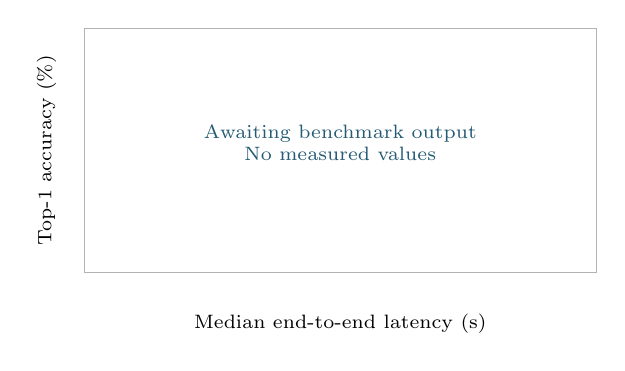
\begin{tikzpicture}[font=\scriptsize]
\draw[gray!60] (0,0) rectangle (6.5,3.1);
\node[align=center,text=accent] at (3.25,1.65) {Awaiting benchmark output\\No measured values};
\node[rotate=90] at (-0.48,1.55) {Top-1 accuracy (\%)};
\node at (3.25,-0.65) {Median end-to-end latency (s)};
\end{tikzpicture}

\caption{Reserved accuracy--latency plot: one measured point per platform/configuration. Use median end-to-end latency and answerable-set top-1 accuracy; show uncertainty where supported. No observations plotted.}\label{fig:tradeoff}
\end{figure}
\begin{figure}[t]\centering
% PLACEHOLDER ONLY: no experimental measurements.
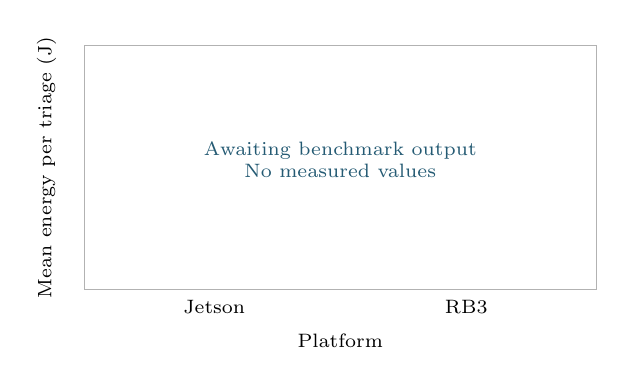
\begin{tikzpicture}[font=\scriptsize]
\draw[gray!60] (0,0) rectangle (6.5,3.1);
\node[align=center,text=accent] at (3.25,1.65) {Awaiting benchmark output\\No measured values};
\node[rotate=90] at (-0.48,1.55) {Mean energy per triage (J)};
\node at (3.25,-0.65) {Platform};
\node at (1.65,-0.22) {Jetson};
\node at (4.85,-0.22) {RB3};
\end{tikzpicture}

\caption{Reserved energy comparison: mean measured joules per triage on the same workload and power boundary, with uncertainty. No observations plotted.}\label{fig:energy}
\end{figure}
\draftnote{Weeks 4--5: explain runtime and quantisation deviations before attributing differences to accelerator hardware. Include p95 latency and measured peak power.}

\subsection{Component ablations}
% PLACEHOLDER ONLY: no experimental measurements.
\begin{table}[t]
\caption{Ablation holders. J/R denotes separate Jetson and RB3 results in each cell. All entries await measurements.}
\label{tab:ablation}\centering\scriptsize
\begin{tabularx}{\columnwidth}{@{}Yccc@{}}\toprule
Configuration & FAR (\%) & Coverage (\%) & Acc@1 (\%)\\\midrule
Full pipeline & --/-- & --/-- & --/--\\
Without keywords & --/-- & --/-- & --/--\\
Without verification & --/-- & --/-- & --/--\\
Without refusal & --/-- & --/-- & --/--\\\bottomrule
\end{tabularx}
\end{table}

\begin{figure}[t]\centering
\input{figures/far.tex}
\caption{Reserved verification ablation: false answer rate with and without verification, for each platform. Report coverage alongside the plotted rate. No observations plotted.}\label{fig:far}
\end{figure}
Ablations use the same frozen incidents and model configuration. Without keyword matching, use vector retrieval alone. Without verification, bypass candidate filtering while retaining schema handling and log raw outputs. Without refusal, use an explicitly defined forced-answer policy; this is an experimental configuration only. Document which stages change and do not silently select a different model. Replay fixed raw candidate outputs where appropriate to isolate verifier effects, and distinguish replay from end-to-end runs.
\draftnote{Week 5: explain whether each component earns its place. Three coarse cause categories can make top-3 accuracy trivial if all are always returned; state the cause taxonomy and examine candidate precision.}

\section{Limitations and Threats to Validity}
\subsection{Evidence sufficiency and annotation}
A deterministic verifier checks specified properties, not unrestricted truth. A valid line reference can accompany an incorrect explanation. Document the reliability of cause labels, disagreement resolution, repeated incidents, and any ambiguity between a reported symptom and the underlying fault. Avoid deriving the answer key from the model being evaluated.
\subsection{External validity and platform matching}
Results on public server logs do not establish semiconductor-test performance. Synthetic cases may be easier than deployment data. A small evaluation set and a narrow cause taxonomy limit generalisation. Runtime, quantisation, cooling, and power-boundary differences may confound a hardware comparison.
\subsection{Observed failure modes}
\placeholder{21mm}{Failure-mode holder\\Record at least three measured categories.\\For each: case IDs, evidence, failure mechanism, mitigation.}
\draftnote{Week 5: replace this holder with actual cases. Candidate categories to investigate include misleading term overlap, missing retrieved evidence, and multi-component ambiguity. These are hypotheses, not observed findings.}

\section{Conclusion and Future Work}
\draftnote{Week 6: answer RQ1--RQ3 using generated results. State the principal accuracy--coverage--energy trade-off and its boundaries. Do not introduce new experiments. Discuss autonomous recovery only as future work unless the optional extension was completed and separately evaluated.}

\section*{Reproducibility and Artifact Availability}
The project repository is available at \url{https://github.com/kaymansrinivasan/air-gapped-rca}. Record the evaluated commit, dataset and model checksums, configuration files, command, raw outputs, and measurement traces. Preserve generated tables and figures with their input records. The current repository is a skeleton; it does not yet reproduce a triage experiment.

\begin{thebibliography}{00}
\bibitem{loghub} LogPAI, ``Loghub: A large collection of system log datasets for AI-driven log analytics,'' dataset repository. [Online]. Available: \url{https://github.com/logpai/loghub}. Accessed: Sep. 7, 2026.
\bibitem{hadoop} LogPAI, ``Hadoop dataset documentation,'' Loghub. [Online]. Available: \url{https://github.com/logpai/loghub/blob/master/Hadoop/README.md}. Accessed: Sep. 7, 2026.
\bibitem{hadooplabels} GitHub contributor mmantyla, ``Incorrect labels in Hadoop log data,'' Loghub, issue 56, Dec. 14, 2024. [Online]. Available: \url{https://github.com/logpai/loghub/issues/56}. Accessed: Sep. 7, 2026.
\end{thebibliography}
% Add verified primary papers before submission; these web sources are a starting set.
\end{document}
